\section{Real-data example: Gender gap in ICU data}
\label{sec:real_example}
The index number problem reflects that the two reference choices for the (N)OBD could yield two different sets of values for the explained and unexplained components. We are not aware of an illustration in the literature that the two directions (for either the OBD or NOBD) can lead to \emph{substantively} different conclusions. 
\textcolor{red}{We now supply such an illustration with real healthcare data.}
%We supply such an illustration next for a real-data analysis in healthcare.

\textbf{Data.} To construct an example, we examine data from the PhysioNet cohort of intensive care unit (ICU) patients collected for a study of in-hospital mortality \citep{goldberger2000physiobank}, where the outcome $Y$ is a binary indicator for whether the patient died in the hospital. The dataset contains routine measurements, including heart rate (HR), mean arterial pressure, and temperature. These values are recorded for every patient at the time of entry into the ICU and provide a description of their initial physiological state. To simulate various real-data analyses where practitioners might have access to only a subset of these patients, we construct $139$ versions of this dataset with various patient subsets; see \cref{appendix:icu_details}.
For reference groups, we consider males and females.

%Medical practitioners often look at moderate elevations in heart rate as a first indication of stress, infection, or concerning changes in blood flow and circulation. In the present example, we restrict our analysis to patients whose admission heart rate lies between the $50$th and $75$th percentiles. This patient set, which we refer to as HR quartile two, reflects a clinical presentation in which the heart rate is elevated but not extreme.

\begin{wraptable}{r}{0.45\textwidth}
%\begin{table}[!ht]
    \label{tab:flip_summary_main}
            \caption{Number of data subsets (out of $139$) exhibiting at least one sign flip (in either the explained or unexplained component), by model. Columns $10\%$, $5\%$, and $1\%$ report the number of flipped subsets that are significant at the corresponding level.}
    \centering
    \small
    \begin{tabular}{lcccc}
    \toprule
    Model & Total flips & $10\%$ & $5\%$ & $1\%$ \\
    \midrule
    Linear      & 27 &  2 &  2 &  2 \\
    Logistic    & 29 &  2 &  2 &  1 \\
    Neural net  & 62 & 29 & 17 &  6 \\
    XGBoost     & 62 & 17 & 10 & 3 \\
    TabPFN     & 76 & 22 & 19 & 5 \\
    \bottomrule
    \end{tabular}

%\end{table}
\end{wraptable}

\textbf{Analysis.}
As discussed in \cref{sec:ob_real}, practitioners often draw conclusions based on the sign and statistical significance of the (N)OBD explained and unexplained components.
To explore whether these conclusions can be robust to the choice of reference group, we compute the explained and unexplained components for each of our $139$ data subsets across one foundation model and four classic models. The foundation model is TabPFN, a $25$ million parameter, transformer-based model, pre-trained to map training datasets to predictive distributions $Y|X$ \citep{hollmann2023tabpfn}. The other four models are linear regression,\footnote{Despite the binary outcome $Y$, it is common practice in applied health and policy research to fit separate linear models (via ordinary least squares) for the relationship between a binary outcome and covariates in each group, and then apply the OBD \citep{jann2008, edokaChangesCatastrophicHealth2017, sujin_LPM_OB, mweembaGapSelfRatedHealth2023}. In fact, this use of the linear model for a binary outcome is so common that it has a name, the ``linear probability model.''} logistic regression, XGBoost \citep{chen2016xgboost}, and a two-layer fully-connected neural network.
% \textcolor{red}{All models are trained and evaluated in-sample. We detail hyperparameter choices in \cref{appendix:icu_details}.}
%To examine a more modern, transformer-based model, we also consider TabPFN, a $25$ million parameter, pre-trained model trained to map training datasets to predictive distributions $Y|X$ \citep{hollmann2023tabpfn}.
We assess statistical significance using $1{,}000$ bootstrap replications.
\cref{tab:flip_summary_main} counts the number of sign flips across these models at various levels of statistical significance.
Concerningly, we see that \emph{every} model contains at least one sign flip, and more complex models tend to have even more flips; for TabPFN, we see that more than  half of the datasets show opposite signs for at least one of the explained or unexplained components, and $13.7\%$ show significant sign flips at the $5\%$ level.



% Within the data set described above, we will compare two patient groups across hospitals (rather than hospital-specific patient groups as in our introductory example). In particular, we let the groups be $g \in \{\text{men}, \text{women}\}$. 
% The mortality rate for men exceeds the mortality rate for women by about $3.5$ percentage points; see \cref{tab:hr_q2_decomposition}.
% We would like to understand to what extent the observed mortality difference between men and women in HR quartile two might be attributable to observed characteristics upon admission (covariates) vs.\ medical care (outcome given covariates). 
% To that end, let $Y$ be a binary indicator for in-hospital mortality, and let $X$ be the vector of admission covariates comprising heart rate, mean arterial pressure, temperature, urine output, age, and ICU type.
% Despite the binary outcome $Y$, it is common practice in applied health and policy research to fit separate linear models (via OLS) for the relationship between a binary outcome and covariates in each group, and then apply the OBD \citep{jann2008, edokaChangesCatastrophicHealth2017, sujin_LPM_OB, mweembaGapSelfRatedHealth2023}.\footnote{In fact, this use of the linear model for a binary outcome is so common that it has a name, the ``linear probability model.''} We provide a detailed description of our data analysis --- and our search procedure for a data analysis exhibiting a substantive conclusion change --- in \cref{appendix:icu_details}. 



\subsection{A deeper dive on one data subset}

\cref{tab:flip_summary_main} shows that sign flips are common.
But what do these flips really mean in practice?
And are they merely an artifact of noise or instead a structural phenomenon?
As is often the case in studying complex machine learning models, studying linear regression provides a tractable proxy problem.
In the present study, linear regression is also of direct interest since the OBD (with linear regression) is widely used in practice.
So, for the rest of the paper, we focus on \cref{eq:OB_H_Counterfactual,eq:OB_K_Counterfactual} with linear regression (i.e., the OBD instead of NOBD).
To start answering our questions, we examine one particular data subset leading to a significant sign flip for linear regression in \cref{tab:flip_summary_main}.
We will see what it means for sign flips to change meaningful conclusions and also see that flips have a natural structural interpretation.

The particular data subset we consider covers patients with an elevated heart rate.
Medical practitioners often look at moderate elevations in heart rate as a first indication of stress, infection, or concerning changes in blood flow and circulation. In the present example, we consider patients whose admission heart rate lies between the $50$th and $75$th percentiles. This patient set, which we refer to as HR quartile two, reflects a clinical presentation in which the heart rate is elevated but not extreme.

\textbf{Two different conclusions.} 
We report the OBD for each reference group in \textcolor{red}{Appendix} \cref{tab:hr_q2_decomposition}. We next interpret the substantive conclusions
we might draw from each reference group. First, consider women as the reference. The explained component is positive ($0.021$), with a statistically significant difference from zero.
This result suggests that differences in admission covariates place men at higher mortality risk. A medical practitioner might therefore examine whether various factors before admission differ across gender; these factors include early differences in blood flow and circulation, underlying disease burden, or overall severity at admission.

Second, consider men as the reference. The explained component is negative ($-0.007$), though the difference from zero is not statistically significant. In this case, the observed covariate differences seem to predict \emph{lower} (or equal) mortality for men relative to women rather than higher. In other words, the same covariates would now be interpreted as offering men a slight mortality advantage. This interpretation is substantively different than the interpretation that results from using women as the reference. 
\textcolor{red}{In \cref{appendix:how-does-flip-arise} we show how differences in linear regression coefficients for men and women lead to this reversal.}

%\begin{table}[h]
%\caption{Oaxaca--Blinder decompositions for HR quartile two. We compute standard errors (in parentheses) via bootstrap resampling with $1{,}000$ replications. 
%    We calculate p-values using a normal approximation (Wald test), where the test statistic is the coefficient divided by its bootstrap standard error. 
%    Significance levels: * $p<0.10$, ** $p<0.05$, *** $p<0.01$.}
%\label{tab:hr_q2_decomposition}
%    \begin{center}
%    \begin{small}
%    \begin{sc}
%    \begin{tabular}{lccc}
%    \toprule
%    \textbf{Reference} & \textbf{Explained} & \textbf{Unexplained} & \textbf{Total gap} \\
%    \midrule
%    %\hline \\[-6pt]
%    Women 
%    & \makecell{$0.021^{***}$ \\ $(0.007)$}
%    & \makecell{$0.014$ \\ $(0.025)$}
%    & \makecell{$0.035$ \\ $(0.023)$}
%    \\
%    Men 
%    & \makecell{$-0.007$ \\ $(0.011)$}
%    & \makecell{$0.042^{*}$ \\ $(0.025)$}
%    & \makecell{$0.035$ \\ $(0.023)$}
%    \bottomrule
%    \end{tabular}
%    \end{sc}
%    \end{small}
%    \end{center}
%\end{table}

%%% MOVED to \cref{appendix:hrq2} (Appendix B.1). To reverse: uncomment below, delete the red copy there.
%REV \begin{table}[!ht]
%REV   \caption{Oaxaca--Blinder decompositions for HR quartile two. The total gap is men's mean minus women's mean. We compute standard errors (in parentheses) via bootstrap resampling with $1{,}000$ replications. 
%REV     We calculate p-values using a normal approximation (Wald test), where the test statistic is the coefficient divided by its bootstrap standard error. 
%REV     Significance levels: * $p<0.10$, ** $p<0.05$, *** $p<0.01$.}
%REV   \label{tab:hr_q2_decomposition}
%REV   \begin{center}
%REV     \begin{small}
%REV       %\begin{sc}
%REV         \begin{tabular}{lcccr}
%REV           \toprule
%REV           Reference & Explained & Unexplained & Total gap  \\
%REV           \midrule
%REV               Women 
%REV     & \makecell{$0.021^{***}$ \\ $(0.007)$}
%REV     & \makecell{$0.014$ \\ $(0.025)$}
%REV     & \makecell{$0.035$ \\ $(0.023)$}
%REV     \\
%REV     Men 
%REV     & \makecell{$-0.007$ \\ $(0.011)$}
%REV     & \makecell{$0.042^{*}$ \\ $(0.025)$}
%REV     & \makecell{$0.035$ \\ $(0.023)$}
%REV     \\
%REV           \bottomrule
%REV         \end{tabular}
%REV       %\end{sc}
%REV     \end{small}
%REV   \end{center}
%REV   \vskip -0.1in
%REV \end{table}

\begin{figure}[!ht]
    \centering
    \begin{subfigure}[t]{0.48\linewidth}
        \centering
        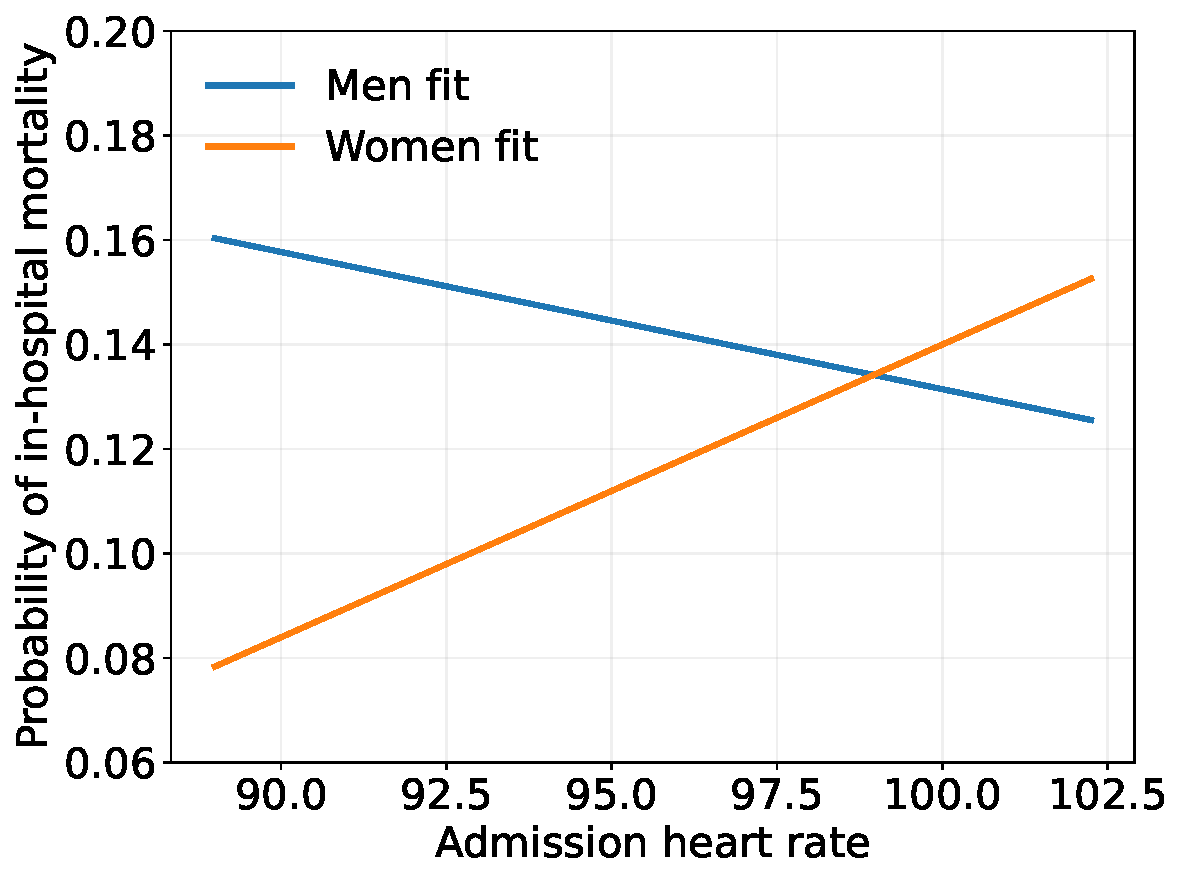
\includegraphics[width=\linewidth]{Sections/Figures/hr_quartile2_mortality_lines.pdf}
        \label{fig:hr_quartile2}
    \end{subfigure}
    \hfill
    \begin{subfigure}[t]{0.48\linewidth}
        \centering
        
\includegraphics[width=\linewidth]{Sections/Figures/prob_unexplained.pdf}
        \label{fig:prob_unexplained}
    \end{subfigure}
    \caption{Left: Linear fit of mortality on admission heart rate for each group when holding all other covariates fixed at their group means. Right: Percentage of parameter space leading to sign flips. See \cref{remark:computing_irwin_hall} for how we compute the percentage for the unexplained component.}
    \label{fig:sign_flip_overview}
\end{figure}


\textbf{Limitations.}
\textcolor{red}{We discuss the limitations of this analysis --- and a second illustration, on U.S.\ Census data, that addresses them --- in \cref{appendix:real_data}.}

%%% MOVED to the head of Appendix B (Sections/09_icu_details.tex). To reverse: uncomment below, delete the red copy there.
%REV \textbf{Limitations.}
%REV Our analysis reveals sign flips in the explained and unexplained components of the (N)OBD in a real dataset.
%REV It is a priori possible that some of our choices may be unusual; these choices include the dataset itself, our choice of covariates, our choice of outcome, or our particular subset of data. And it is possible that sign flips may not occur in other settings.
%REV To address this possibility, we provide a second illustration analyzing differences in income as well as health insurance status using U.S.\ Census data in \cref{appendix:us_labor_force}.
%REV The latter data have previously been analyzed by \citet{bach2024heterogeneity}, reducing the concern that our empirical results are due to atypical choices on our part.
%REV We also give a theoretical account of sign flips in \cref{sec:signflips}, where we establish that they correspond to a nontrivial region of the parameter space.